\section{Requirements Engineering}

\begin{tcolorbox}[title=Requirements Engineering]
    \textbf{Requirements Engineering} ist das systematische Vorgehen des Ermittelns von Anforderungen,
    wobei mit möglichst geringem Aufwand alle notwendigen Informationen gesammelt und schriftlich festgehalten werden.
\end{tcolorbox}

\begin{figure}
    \centering
    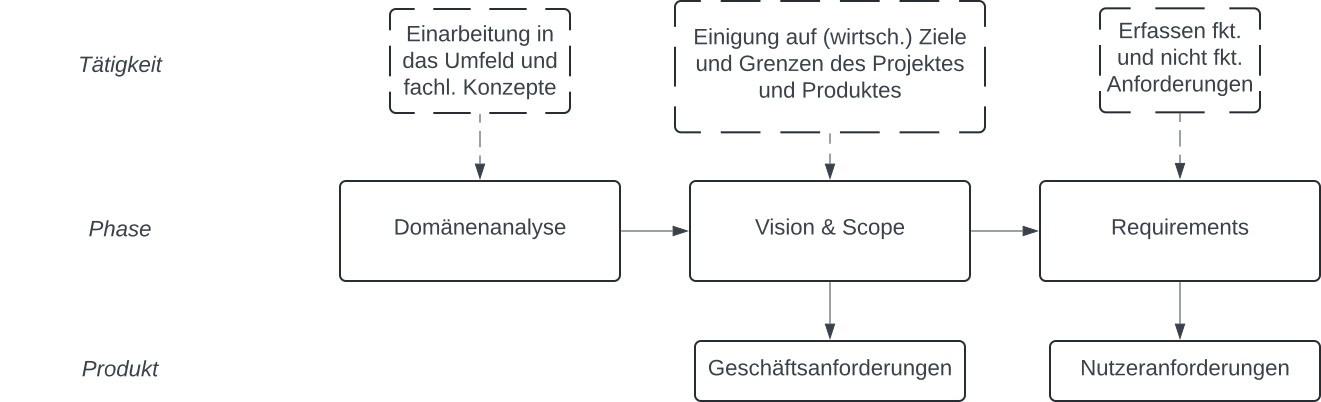
\includegraphics[scale=0.35]{chapters/Anhang/CheatSheets/img/requirementsengineering}
    \caption{Phasen des Requirement Engineerings sowie deren Tätigkeiten und Ergebnisse. (Quelle: in Anlehnung an~\cite[84]{Wed09})}
    \label{fig:requirementsengineering_cc}
\end{figure}

\begin{figure}
    \centering
    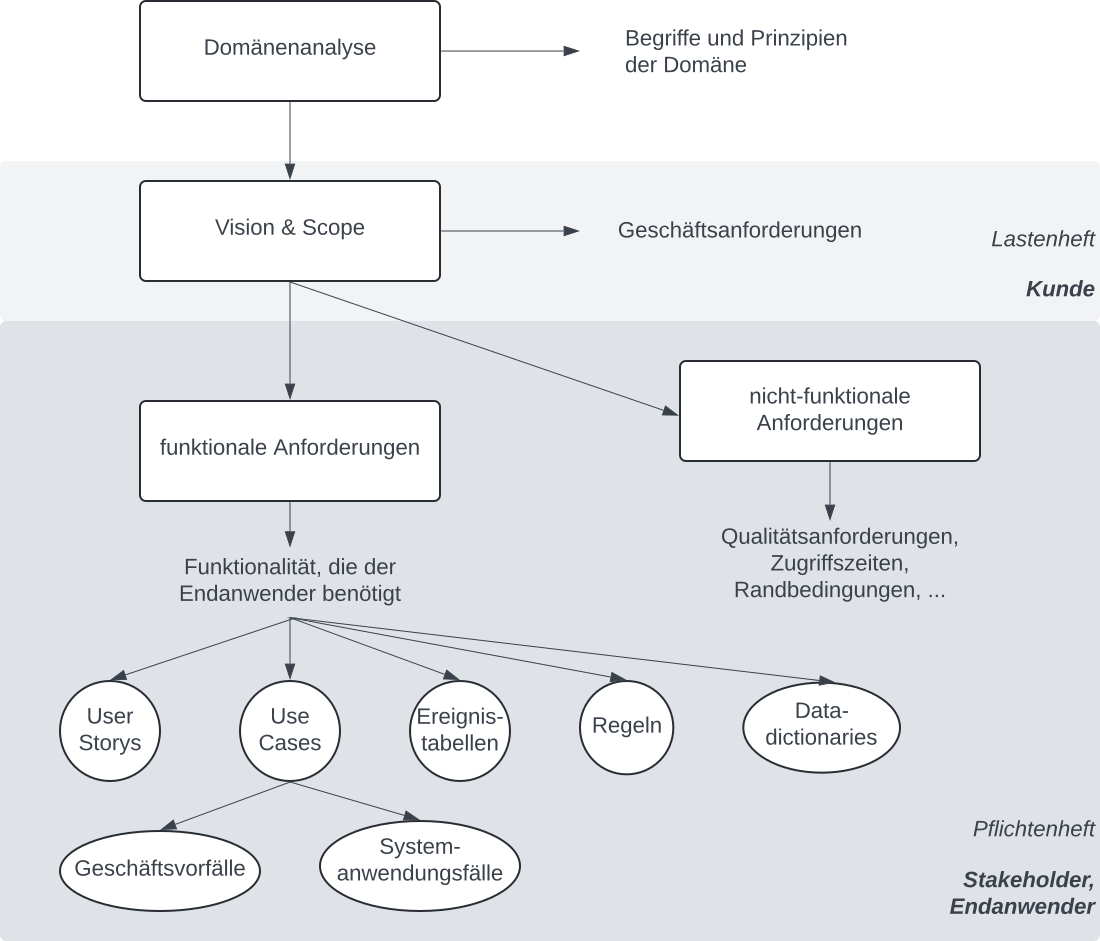
\includegraphics[scale=0.35]{chapters/Anhang/CheatSheets/img/anforderung}
    \caption{Abfolge der Erfassung verschiedener Anforderungen. (Quelle: eigene)}
    \label{fig:anforderung_cc}
\end{figure}